\startchapter{Deformable Model}
\label{chapter:deformablemodel}
Interactive visualization techniques developed in the previous chapters support a \blob based modelling 
system for the incremental construction process. In a surgical simulation scenario, tissues undergo 
various levels of deformations and topological modifications. Researchers in the field studied different 
approaches to recreate the elastic behavior of tissues. The two main challenges that are reported 
continuously in this field are interactivity and fidelity of motion \cite{Meier2005}. 

Based on the foundation built so far, we build a deformable model to support 
the required interactions with surgical tools i.e., elastic deformations by pushing the tissue. 
The next chapter will address the problem associated with cutting, which is a primary operation in 
many surgical simulation scenarios. The goal is to make a comprehensive system that bridges the gap 
between modelling and simulation of tissues. 

\section{Overview}
A software pipeline is developed to support physically based simulation of deformable tissues using our 
implicit modelling framework, figure \ref{fig:systempipeline}. 

\begin{figure}[H]
  \centering
  % the following command controls the width of the embedded PS file
  % (relative to the width of the current column)
  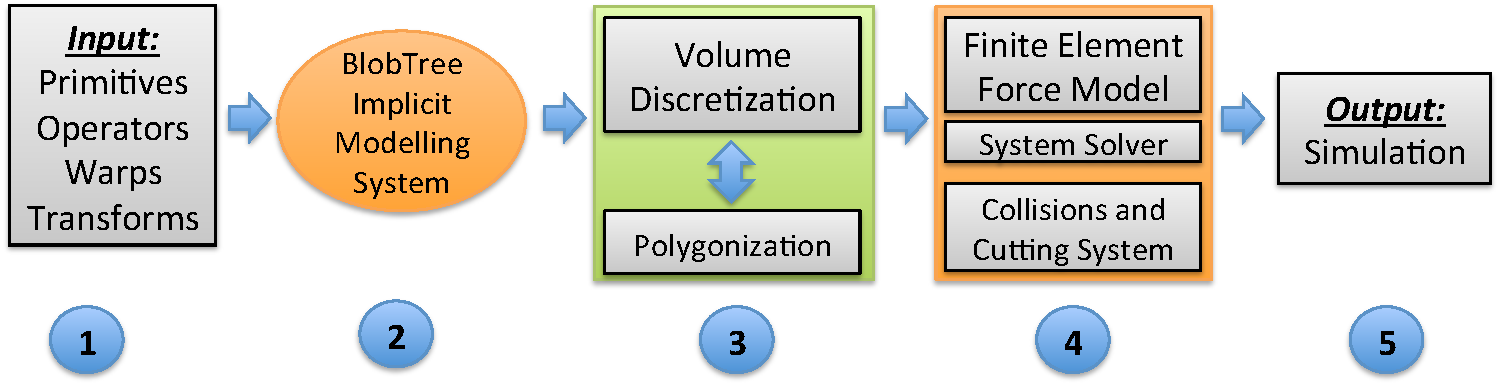
\includegraphics[width=1.0\linewidth]{figures/deformable/pipeline.pdf}
  \caption{\label{fig:systempipeline}
  {High-level system software pipeline to support deformations and cutting. }
}
\end{figure}

Stages 1 and 2 in the pipeline are associated with the modelling process which is 
already discussed in section \ref{sec:implicitmodellingintro}. Stage 3 is 
associated with the polygonization algorithms that are developed in chapters \ref{chapter:cpuPoly} 
and \ref{chapter:GPUDiscretization}. Also in stage 3 is the volume discretization technique that converts 
the \blob model into a tetrahedral mesh for physical simulation, this process is discussed further in 
section \ref{sec:physicalmodel}. The material that is discussed in the current and the next chapters are associated with the 
stage 4 of the pipeline shown above. The output of the system is the simulation environment that 
facilitates deformations and cutting which is shown as the final stage of the pipeline. 


\section{Physical Model}
\label{sec:physicalmodel}
The deformable model has to be considered as a continuous volume in order to reproduce its elastic, 
volumetric effects. In our system, the \blob model is discretized into a tetrahedral mesh using the 
algorithm proposed by Labelle \etal \cite{Labelle2007}. This is a one time process 
and is not a bottleneck in our system. 


A fine-grained cell-size parameter captures the exterior part of the model while a coarser sampling is 
used to produce the internal tetrahedral cells. This approach allows us to maintain a balanced number 
of tetrahedral cells for the physics simulation. The output of this stage is called \textit{volume mesh} in 
order to differentiate it from the surface mesh which is extracted using the polygonization algorithm in 
the previous chapters. The data structure representing the tetrahedral meshes in our system is described in section 
\ref{sec:tetmeshstructure}.

%describe our finite element force model


\section{Deformations}





 




















